\documentclass[a4paper,12pt]{article}
\usepackage[utf8]{inputenc}
\usepackage[T1]{fontenc}
\usepackage[spanish]{babel}
\usepackage{csquotes}
\usepackage{anysize}
\usepackage{graphicx}
\marginsize{25mm}{25mm}{25mm}{25mm}

\title{Delays to food-predictive stimuli do not affect suboptimal choice in rats}
\author{Paul J. Cunningham \and Timothy Shahan}
\date{2020}

\begin{document}
{\scshape\bfseries \maketitle}

Existen ejemplos de susceptibilidades maladaptativas que son difíciles de reconciliar con teorías normativas. El estudio de las decisiones maladaptativas puede proveer nuevas perspectivas en el tipo de información que los animales usan para tomar decisiones.

Un ejemplo es la elección en el procedimiento de elección subóptima.

La investigación indica que la elección subóptima sucede debido a que las palomas toman decisiones basadas en la relación predictiva entre el estímulo del TL y la comida, en lugar de en la probabilidad de entrega de comida, {\itshape i.e.,} las palomas se ven más atraídas por los estímulos predictores. Se trata de una decisión maladaptativa en la cual las palomas sacrifican comida para recibir información sobre ella. Estudiar estas elecciones puede dar luz sobre la forma en que los estímulos predictores influyen en la toma de decisiones.

Se ha propuesto que la elección subóptima también puede aportar perspectivas sobre las decisiones maladaptativas en la conducta de juego patológico en humanos.

Se ha fallado en varias ocasiones en encontrar elección subóptima en ratas, pero Cunningham y Shahan (2019) mostraron que las ratas muestran elección subóptima cuando la demora a la comida es suficientemente larga. Cuando la duración del TL era de al menos 30s, las ratas mostraron elección subóptima.

Este resultado fue predicho por el modelo {\itshape temporal information-theoretic approach}. Este modelo puede informar a los experimentos en ratas y proveer conceptos cuantitativas para interpretar las diferencias potenciales entre las elecciones de ratas y palomas. El modelo está formado por tres partes:

\begin{enumerate}
	\item Los estímulos del TL influyen la elección con base en la información temporal que proveen (sobre {\itshape cuándo} se espera la comida). Esto se deriva del papel de la información temporal en el condicionamiento pavloviano, y del papel de los estímulos predictores de comida para influir en la conducta operante. La información temporal se cuantifica aplicando la medida de incertidumbre de Shannon a las distribuciones de probabilidad de (1) los intervalos entre entregas de comida y (2) los intervalos entre el encendido del estímulo y la entrega de comida.

		La incertidumbre basal depende del intervalo medio entre entregas de comida independientemente de otras claves. La incertidumbre media sobre cuándo esperar comida en presencia de un estímulo depende del intervalo medio entre su encendido y la entrega. La información temporal dada por el estímulo se mide comparando ambas incertidumbres:

		\begin{equation}
			H = 
			(log_{2}C+k)
			-
			(log_{2}t+k)
			=
			log_{2}(C/t)
		\end{equation}
		donde $H$ representa los bits de información temporal dados por el estímulo, $C$ es el intervalo entre comida, $t$ es el intervalo estímulo-comida, y $k$ es una constante que depende de la resolución temporal de los animales. Estímulos que señalan una mayor reducción en la demora proveen más información temporal.

		Las palomas deberían preferir la alternativa que ofrece más información temporal según la ecuación 

		\begin{equation}
			\frac{
				H^{a}_{Sub}
			}{
				H^{a}_{Sub} + H^{a}_{Opt}
			}
		\end{equation}
		donde $a$ es la sensibilidad de la elección a la información temporal relativa. Cuando la alternativa subóptima tiene estímulos que señalan diferencialmente la comida, el $S^{+}$ provee más información temporal que los estímulos de la alternativa óptima. Esto captura la razón por la cual el $S^{+}$ atrae más respuestas. Según este modelo, los estímulos nunca seguidos de comida no tendrán contribución en el valor relativo de las alternativas. Esto es consistente con estudios que muestran que ni la duración ni la probabilidad del $S^{-}$ tienen efecto en la elección de las palomas.
	\item La tasa de entrega de comida también influye la elección de acuerdo con la ley de igualación:

		\begin{equation}
			\frac{
				R^{b}_{Sub}
			}{
				R^{b}_{Sub} + R^{b}_{Opt}
			}
		\end{equation}
		donde $R$ es la tasa de entrega de comida para las alternativas y $b$ es la sensibilidad a la tasa de entrega de comida. Las palomas deberían preferir la alternativa con tasa más alta (la óptima). La información temporal y la tasa de entrega compiten para controlar la elección:

		\begin{equation}
			pSub = 
			w \frac{
				H^{a}_{Sub}
			}{
				H^{a}_{Sub}+H^{a}_{Opt}
			} +
			(1-w)
			\frac{
				R^{b}_{Sub}
			}{
				R^{b}_{Sub} + R^{b}_{Opt}
			}
		\end{equation}
		donde $w$ da el peso dado a cada componente. La información temporal sesga hacia la elección subóptima, y la tasa de recompensa hacia la óptima. Cuando $w$ es mayor hay mayor grado de elección subóptima.
	\item La tercera parte es el mecanismo de ponderación $w$ y se basa en estudios que miden la influencia de las duraciones de IL y TL en la elección subóptima. Duraciones mayores de TL llevan a mayor grado de conducta subóptima. Con base en ello el modelo asume que la demora contribuye a la competencia entre los dos componentes.
		
		Aun no es tan claro si el IL influye de la misma forma en la elección. Hay evidencia limitada que indica que IL más largos disminuyen el grado de conducta subóptima. Por tanto algunas teorías no incluyen en absoluto al IL. Aun así, este modelo da cuenta de más datos de palomas si se asume que demoras más grandes al estímulo (mediante IL mayores) disminuyen la elección subóptima afectando el grado de competencia entre los componentes.

		Se asume que el mecanismo ponderador es gobernado por la demora promedio a la comida en el momento de la elección con relación a la demora promedio al estímulo temporalmente informativo en el mismo momento (el momento de elección es el momento en que se presenta la elección al animal):

		\begin{equation}
			w = 
			\frac{
				1
			}{
			1 + e^{-\beta \left(\frac{
				D_{f}
			}{
				D_{s}
			} - m \right)}
			}
		\end{equation}
		donde $D_{f}$ denota la demora promedio a la comida en el momento de la elección, $D_{s}$ denota la demora promedio al estímulo temporalmente informativo en el mismo momento, $\beta$ representa la sensibilidad de $w$ a variaciones en $\frac{D_{f}}{D_{s}}$, y $m$ representa el valor de $\frac{D_{f}}{D_{s}}$ en el cual $w = 0{.}5$.
		
		Según incrementa la duración de TL, la demora promedio a la comida en el momento de elección ($D_{f}$) incrementa mientras la demora al estímulo ($D_{s}$) permanece igual. Por lo tanto, TL mayores resultan en $\frac{D_{f}}{D_{s}}$ mayores, y por lo tanto en mayor peso asignado a la información temporal. Mientras incrementa IL sucede lo contrario. Por lo tanto, {\itshape la elección subóptima emerge cuando los estímulos de la alternativa subóptima dan más información temporal, y cuando los estímulos temporalmente informativos están mucho más cerca en el tiempo que la comida en el momento de la elección}.
\end{enumerate}

Aunque se mostró que con TL largos las ratas muestran elección subóptima, no queda claro si esto se debe al impacto de $\frac{D_{f}}{D_{s}}$. No se ha explorado el efecto de la duración del IL en la elección subóptima en ratas. Así, este experimento pretende determinar si el mecanismo de ponderación de las ratas es gobernado por $\frac{D_{f}}{D_{s}}$ o solo por $D_{f}$.

Se dio a las ratas a elegir entre las alternativas usuales variando las duraciones de IL y TL entre condiciones. Dos condiciones tenían un IL con FR 1 y con TL de 10 y 50s, replicando las duraciones mayor y menor de Cunningham y Shahan. Una tercera condición medía la elección subóptima con un IL de IF 5s y un TL de 50s, pero con un valor de $\frac{D_{f}}{D_{s}}$ igual al de la condición de TL de 10s (con un IL más largo). Si la razón $\frac{D_{f}}{D_{s}}$ gobierna el mecanismo de ponderación, esta tercera condición resultará en elección idéntica a la de TL 10s. Si solo importa la demora a la comida ($D_{f}$), las ratas preferirán la alternativa subóptima en la tercera condición dado que la demora será lo suficientemente larga. Por último, una cuarta condición midió la elección subóptima con un IL de FI 10s con TL 50s para determinar si decrementos en $\frac{D_{f}}{D_{s}}$ disminuyen la elección subóptima.

{\scshape\bfseries Method}

Las cajas tenían dos palancas retráctiles con luces equidistantes a un comedero central.

Los estímulos de ambas alternativas fueron estímulos compuestos de luz constante/parpadeante + tono de la misma naturaleza.

El procedimiento difiere del estándar en que (1) se utilizó un blackout como $S^{-}$ de la alternativa subóptima, y (2) solo se usó un estímulo en la alternativa óptima.

Las sesiones tenían 48 ensayos forzados y 24 libres. Cada ensayo inició con una respuesta en el comedero para centrarla. La respuesta de elección era la presión a una de las palancas, y la entrada en el TL era señalada por su retracción. El compuesto de tono+luz se presentaba en la alternativa subóptima si se entregaría comida, de lo contrario la caja permanecía oscura. En la alternativa óptima el estímulo compuesto siempre se presentó. El TL terminaba con la entrega de un único pellet o un blackout de 3 segundos. En las condiciones con IL de intervalo fijo, una respuesta en una de las palancas antes del cumplimiento del tiempo del FI resultaba en la retracción de la otra palanca. Hubo un ITI de 10s entre los ensayos.

Las ratas pasaron por las cuatro condiciones (figura 1).

\begin{figure}[ht]
	\begin{center}
		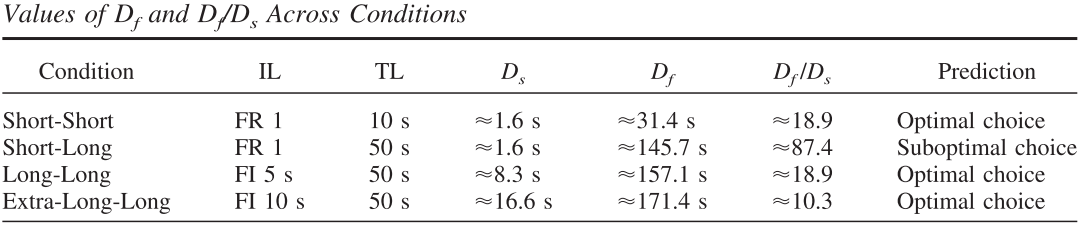
\includegraphics[scale=0.4]{Cunningham2020(1).png}
		\caption{Cuatro condiciones y sus predicciones.}
	\end{center}
\end{figure}

Las condiciones {\itshape short-short} y {\itshape short-long} son replicaciones de Cunningham y Shahan (2019). {\itshape Extra-long-long} se presentó al final para todas las ratas, y las demás fueron contrabalanceadas. Cada condición duró al menos 20 sesiones. {\itshape Long-long} y {\itshape extra-long-long} pretendía determinar si (1) IL más largos reducen la elección subóptima como ocurre en palomas y (2) si la elección subóptima es gobernada por la razón $\frac{D_{f}}{D_{s}}$. Esa razón es idéntica en {\itshape short-short} y en {\itshape long-long}, y es más pequeña en {\itshape extra-long-long}, por lo que en {\itshape long-long} se predice el mismo grado de optimalidad, y en el segundo un grado aun mayor.

{\scshape\bfseries Results}

Las ratas discriminaban bien (visto por entradas a comedero). Hubo un grado mucho mayor de elección subóptima en {\itshape short-long}, {\itshape long-long}, y {\itshape extra-long-long} comparadas con {\itshape short-short}. Esto indica que incrementar la demora a la comida en el momento de la elección incrementa la elección subóptima, aunque pruebas t mostraron que en ninguno de los casos se excedió la indiferencia, pero esto es subóptimo en sí mismo. No hubo diferencias entre las tres últimas condiciones (figura 2), es decir, sin importar las duraciones de IL las ratas mostraron preferencias equivalentes.

\begin{figure}[ht]
	\begin{center}
		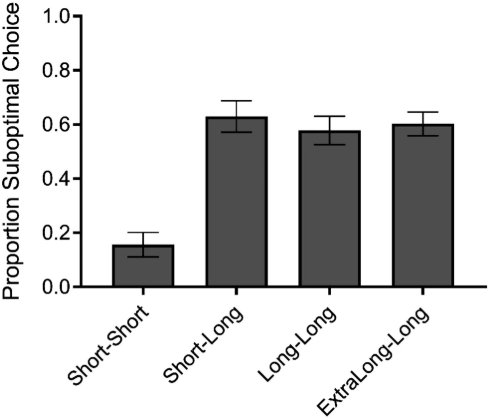
\includegraphics[scale=0.4]{Cunningham2020(2).png}
		\caption{Proporciones de elección por condición. Media de las últimas cinco sesiones.}
	\end{center}
\end{figure}

Comparando las condiciones individualmente con {\itshape short-short} se esperaría con base en el modelo con mecanismo de ponderación basado en la ecuación 5 (1) mayor elección subóptima para {\itshape short-long}, misma elección subóptima para {\itshape long-long}, y menor para {\itshape extra-long-long}. Por lo tanto {\itshape hay poca evidencia que indique que duraciones mayores de IL menguan el incremento en elección subóptima}.

El modelo fue ajustado a todos los datos encontrados además de los datos originales de Cunningham y Shahan. Al incluir todos los datos el modelo solo explicó el 59\% de la varianza, lo que no sorprende dado que los resultados indican que la elección de las ratas no es sensible a $D_{s}$. Parece ser que el mecanismo de ponderación de las ratas no es gobernado por $\frac{D_{f}}{D_{s}}$. 

Quizá un ajuste del mecanismo de ponderación que incluya solo a $D_{f}$ ejecutaría mejor. Si el mecanismo se define como 

\begin{equation}
	w = 
	\frac{
		1
	}{
		1 + e^{
			-\beta(D_{f} - m)
		}
	}
\end{equation}
el modelo explica el 85\% de la varianza. Así, para reconciliar a los datos con el modelo se puede asumir que el mecanismo de ponderación de las ratas es solo gobernado por la demora a la comida en el momento de la elección.

{\scshape\bfseries Discussion}

La evidencia indica que ambas especies necesitan de demoras grandes a la comida para producir elección subóptima. Sin embargo el grado de elección subóptima fue levemente menor aquí que en Cunningham y Shahan (2019), y hubo mayor variabilidad entre sujetos, quizá por la edad de las ratas.

El resultado principal, que la duración del IL no tiene efecto en la elección subóptima, puede ser relevante para las teorías existentes de elección subóptima, y puede sugerir una diferencias en las variables que la gobiernan entre ratas y palomas.

La evidencia del efecto del IL en palomas viene de pocos experimentos, algunos de los cuales han sido criticados por sus peculiaridades procedimentales. Y más aún, el efecto no siempre se encuentra y hay gran variabilidad entre sujetos. Por lo tanto, algunas teorías, como la del valor predictivo de Zentall y la de decaimiento de asociabilidad, no incluyen a los IL.

Otras hipótesis, como la SiGN, le dan un papel crítico. Según esta hipótesis, introducir programas de intervalo en el IL incrementa el valor como reforzador condicionado de los estímulos del TL debido a que la respuesta de elección en el IL se vuelve menos predictiva de la comida. Debido a que incrementos en el IL incrementan el valor reforzador condicionado de las dos alternativas, la diferencia entre ellas se hace relativamente menor, con lo que la elección pasaría a ser mayormente determinada por el otro factor diferente: la diferencia en la tasa de reforzamiento primario.

Aunque parece ser que estos resultados contradicen la hipótesis SiGN, lo cierto es que ésta aun no esta bien especificada, de modo que es difícil hacer comparaciones concretas.

La {\itshape temporal information-theoretic approach} ofrece una perspectiva más concreta. Indica que el grado de competencia entre la información temporal y el reforzamiento primario puede ser distinto entre las especies.

¿Por qué la diferencia estaría en el mecanismo de ponderación? Sería difícil pensar que existe una diferencia en la influencia de la tasa de entrega de comida, pues la ley de igualación es una de las descripciones de elección más generales. En el caso de la información temporal, este proceso está gobernado por reacciones pavlovianas a los estímulos, de modo que sería improbable que exista una diferencia en lo que aprenden los animales sobre los estímulos predictores. Aunque Case y Zentall han mostrado que aun si ambas alternativas aportan la misma información temporal, un grado de elección subóptima se desarrolla lentamente, lo que es explicado como un proceso de contraste y sale del alcance de este modelo.

Así, el candidato probable es el mecanismo de ponderación. La evidencia presente indica que ratas y palomas podrían tener un mecanismo distinto. Si se asume que el mecanismo de las ratas solo toma en cuenta $D_{f}$ entonces el ajuste es bastante bueno.

Dado que la evidencia que apoya a la inclusión del IL en el caso de las palomas es débil, quizá el modelo funcionaría bien también en ellas si solo se considera a $D_{f}$ en el mecanismo de ponderación.

Se intentó ajustar los datos previos de palomas con este nuevo modelo y el resultado fue pobre: se sobre-predecía sistemáticamente la elección subóptima cuando los IL son largos. Por lo tanto, {\itshape el mecanismo de ponderación parece ser necesariamente diferente para ratas y palomas}.

Que las ratas no sean afectadas por la demora a los estímulos no es la única posibilidad. Una alternativa se relaciona con una diferencia procedimental entre este y otros experimentos con palomas: la mayoría de la investigación que mostró menor suboptimalidad con IL más largos tenía estímulos de TL que daban la misma cantidad de información temporal para cada alternativa ({\itshape e.g.,} elección entre una alternativa subóptima que daba 50\% de comida con estímulos discriminativos y una alternativa óptima que daba comida siempre). En estas condiciones, con duraciones de IL cortas el modelo predice indiferencia dado que la información temporal de los TL no favorece a ninguna alternativa. Mientras la duración de IL incrementa, $w$ tiende a cero y se espera preferencia por la alternativa óptima. Pero en el experimento actual y otros recientes el $S^{+}$ provee más información temporal que los estímulos de la alternativa óptima. Aquí el modelo predice preferencia por la alternativa subóptima con IL cortos, y reversión con IL más largos. Colocar un estímulo relativamente más informativo en la alternativa subóptima no debería afectar la influencia de la duración del IL en la elección subóptima. Solo debería permitir un cambio a la suboptimalidad cuando $w$ tiende a 1 en lugar de tener un techo en la indiferencia. Es decir, el modelo asume que las variables que gobiernan al mecanismo de ponderación ($D_{f}$ y $d_{s}$) no interactúan entre sí.

Pero es posible que el efecto de la duración del IL dependa de la información temporal dada por los estímulos del TL, es decir, que sí exista una interacción de modo que IL afecte a la elección subóptima solamente cuando los estímulos del TL son igualmente valorados por su información temporal. No hay evidencia al respecto, pero este tema potencialmente llevaría a la reestructuración del modelo.

Un siguiente paso razonable sería comparar la elección subóptima en un rango de duraciones de IL cuando los estímulos de cada alternativa provean de la misma o distinta información temporal.

Si las ratas son de hecho insensibles a la duración del IL sin importar la información temporal la siguiente pregunta será por qué lo son. Una posibilidad es que su sensibilidad a la duración del IL dependa del grado de saliencia incentiva adquirida por el estímulo del TL. Sin embargo, se ha mostrado que la saliencia incentiva no es necesaria ni suficiente para producir elección subóptima, pero es posible que juegue un papel más sutil: podría traducirse en el sesgo de un animal para utilizar los estímulos predictores para realizar elecciones o en la sensibilidad a las variaciones en $\frac{D_{f}}{D_{s}}$ o solo a $D_{f}$. Podría influir en la demora a la comida requerida para sesgar a los animales a usar la información temporal para tomar decisiones.

Este experimento utilizó luces y sonidos, que tienen menor saliencia para las ratas que la que las teclas tienen para las palomas. Esta posibilidad podría explorarse variando la duración del IL usando luces o palancas como estímulos. Se esperaría que IL más largos decrementarían la elección subóptima al usar palancas.

No está claro por qué las demoras a los eventos relevantes para la decisión deberían gobernar el mecanismo de ponderación. Una posibilidad es un proceso atencional. Las demoras podrían gobernar la atención prestada a la comida y a los estímulos que la predicen, afectando su impacto en la elección. El mecanismo también podría reflejar un proceso de aprendizaje en que los animales asignan crédito de los resultados a sus elecciones. En este caso las demoras influirían en la habilidad de los animales para determinar que elecciones llevaron a qué consecuencias. Pero es necesaria más investigación.

Este experimento replicó el efecto de que demoras mayores a la comida (mayores TL) llevan a elección subóptima en ratas. El experimento sugiere que incrementar la demora a los estímulos (mayores IL) no afecta a la elección subóptima en ratas. Esto sugiere la existencia de mecanismos de ponderación distintos entre las especies. Pero aun se requiere investigación para aclarar (1) si y cómo la duración del IL influye en la elección subóptima, y (2) si hay diferencias en el papel del IL entre las especies.


\end{document}
